
%Copyright (C) 2016 by Krishneel@JSK Lab, The University of Tokyo

\documentclass{standalone}

\usepackage{hyperref}
\usepackage{footnote}
\usepackage{graphicx}

\begin{document}

\subsection{Hardware}
Our robot consists of an upper body humanoid(hrp2) on a high-power mobile base(Fig.\ref{fig:figure1}). The robot is equipped with a stereo camera, a long range laser sensor, a global positioning system (GPS), and a custom made gripper. The gripper consists of a magnet embedded link actuated by a servo motor as shown in Fig.\ref{fig:figure2}. The wrist is also equipped with a six axis force torque sensor.

The hrp2 is our lab's main robot, it is relatively mature and we have created a lot of software packages for this robot, like the lisp based program language euslisp. For the moving base, we bought the base and designed both the control hardware circuits and the ROS control interface for the moving base.


\begin{figure}[t]
  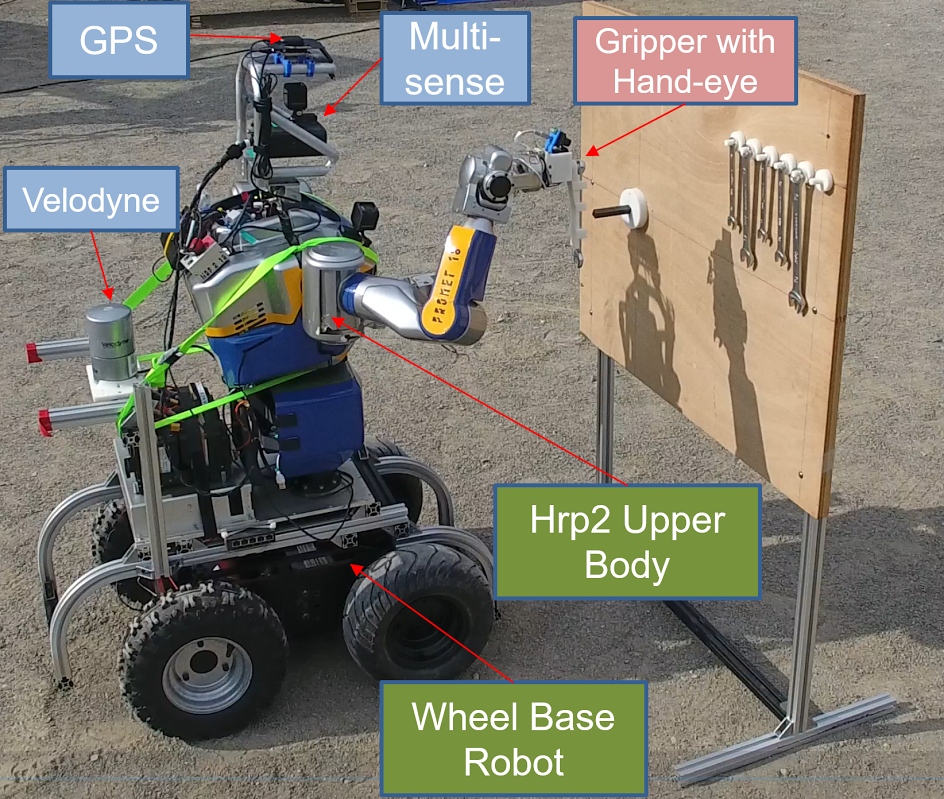
\includegraphics[width=\columnwidth]{sections/task2/images/hrp2}
  \caption{HRP2 robot platform for task2}
  \label{fig:figure1}
\end{figure}

\subsection{Software}

For task 2, the softwares are also implemented on ROS environment with utilization of multithreading for fast computation. Euslisp programming language from JSK lab was used for kinematics simulation and robot control. OpenCV and in-house developed algorithms
 \footnote{\url{https://github.com/jsk-ros-pkg/jsk_recognition}} are used for recognition and perception.


 \subsection{General Approach}
 \textbf{Navigation}: Our approach is to use the long range laser sensor and the GPS for searching and navigating to the panel when the robot is far from the robot and is out of range for the stereo camera. As the panel becomes closer than the minimum range of the laser sensor, the robot will then switch over to use the stereo camera. Our high-powered mobile base can reach up to 4m/s and can drive through various outdoor terrains. 

\textbf{Wrench and valve stem detection}: We experimented and compared infrared camera with stereo camera, and we have decided to use stereo camera for close range perception, since infrared cameras tend to fail in outdoor sunny environments, and cannot sense objects that are too close to the robot. 

We detect the wrench by using Edge detection, Hough transform and K-means. Firstly, we select a region include 6 wrenches on the camera image(Fig.\ref{fig:figure3}A). We apply hough line transform to the edge image of selected region and extract lines which have large slope, then apply K-means(K is 6) to extracted lines. The size of wrenches can be estimated from classified lines, but the position of wrenches estimated from lines is not correct(Fig.\ref{fig:figure3}B). Therefore we use Hough circle transform to detect the hanger on image(Fig.\ref{fig:figure3}C) and get depth from point cloud(Fig.\ref{fig:figure3}D). Thus, we can detect the size and position of wrenches.  

We also select the region on the camera image to detect the valve stem(Fig.\ref{fig:figure3}A). We estimate the plane from the point cloud in the selected region, extract the points witch exist in front of the plane(Fig.\ref{fig:figure3}E). The centoroid of the extracted points is considered as the position of the valve stem(Fig.\ref{fig:figure3}F).

\textbf{Picking the wrench}: Our robot picks up the wrench by aligning the gripper with the wrench, moving the gripper toward the wrench, and letting the magnets pull the wrench into the gripper. The gripper is designed so that the wrench is grasps firmly, but with some movement possible for passive compliance.

\textbf{Wrench fitting and turning}: To fit the wrench head onto the valve stem, we use force feedback from the wrist to gauge the tool contact state. The robot first moves its gripper above the detected position of the valve stem. Due to error in detection or calibration, the wrench head could be directly above the valve stem or it can be slightly misaligned (Fig.\ref{fig:figure3}A, B). The robot moves its gripper down, until a force in the vertical direction is detected, indicating that the wrench has come in contact with the valve stem. Once it detects contact with the valve stem, the wrench can be in one of the contacts states as shown in Figure 1 The robot then moves its gripper in the horizontal direction in a widening zigzag pattern. Depending on the forces it detects, the robot then begins to turn the wrench, or adjusts its gripper position and retries to fit the wrench (Fig.\ref{fig:figure3}).

\begin{figure}
  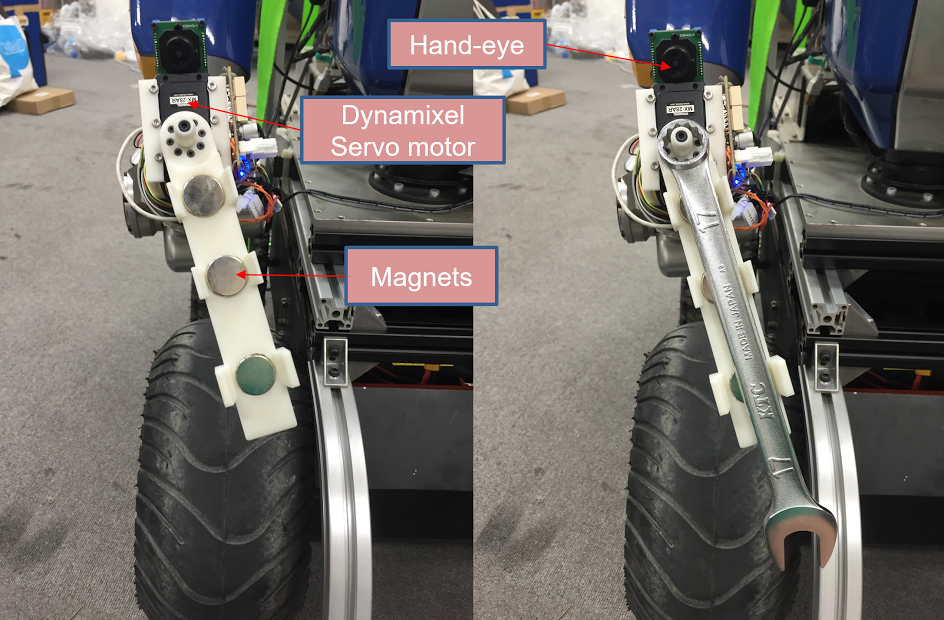
\includegraphics[width=\columnwidth]{sections/task2/images/gripper}
  \caption{Custom made magnetic gripper.}
  \label{fig:figure2}
\end{figure}


\begin{figure}
  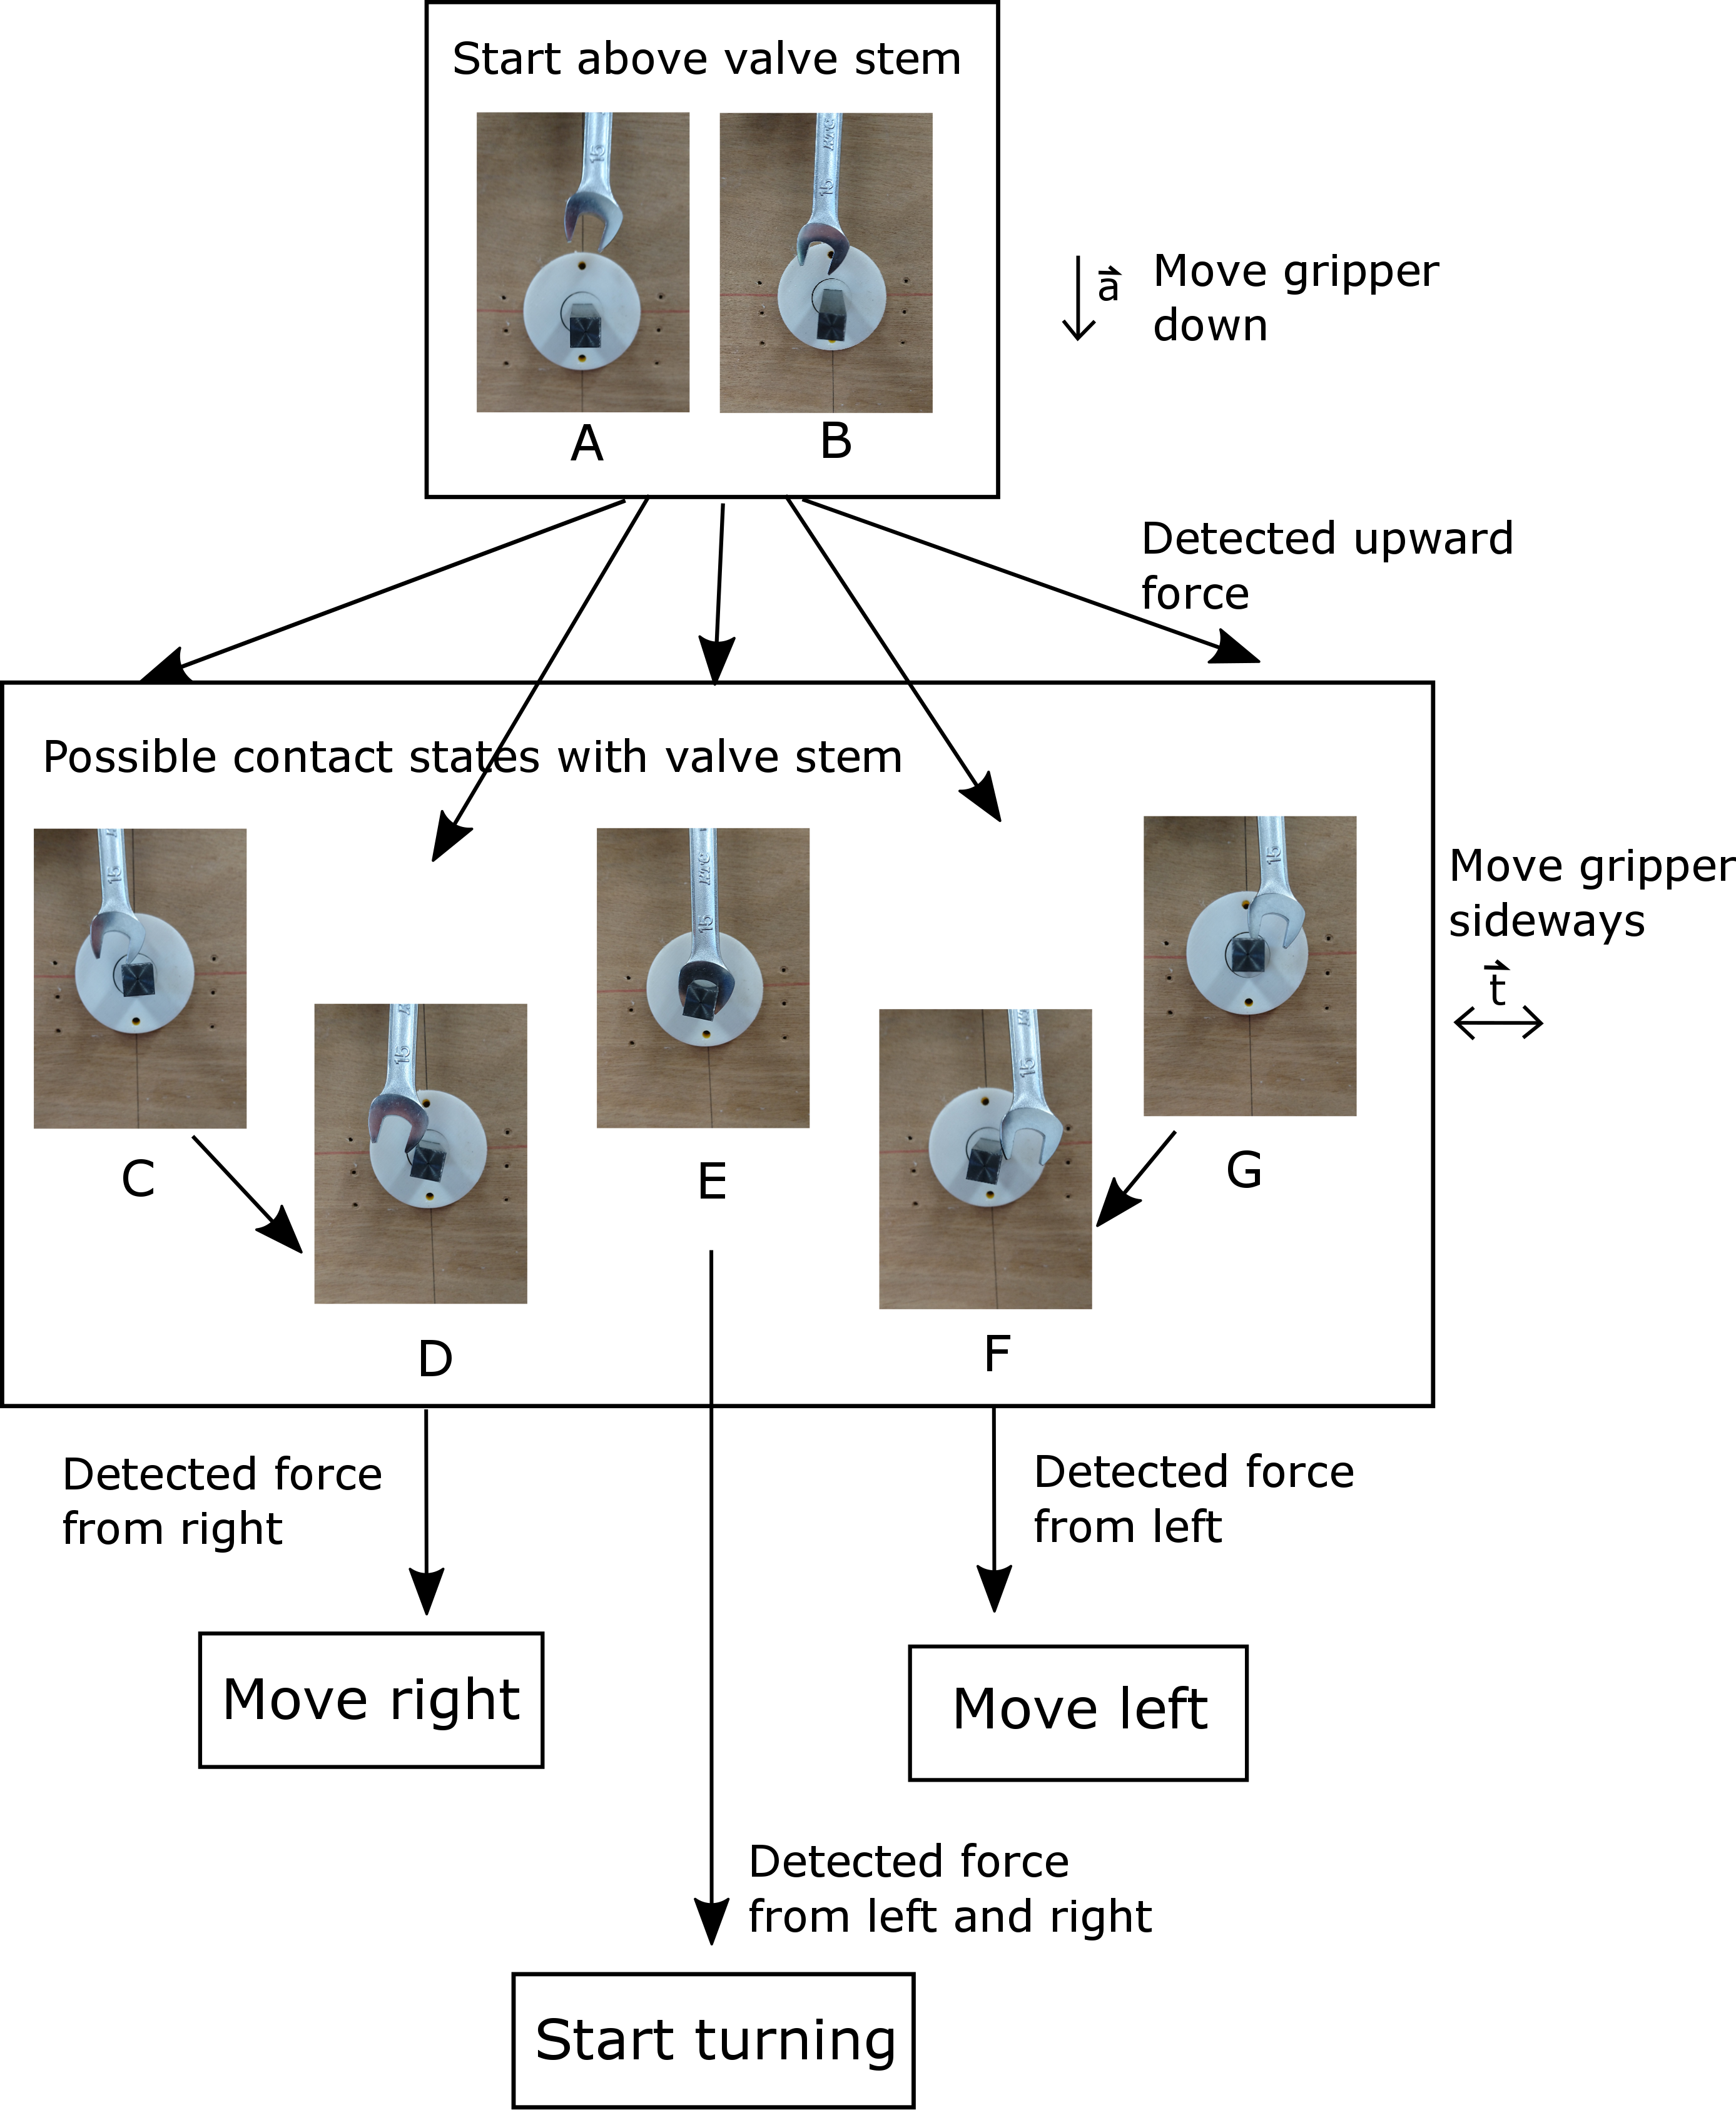
\includegraphics[width=\columnwidth]{sections/task2/images/figure4}
  \caption{Using force fitting for wrench fitting}
  \label{fig:figure3}
\end{figure}


\subsection{Results Achieved to Date}
We have completed the prototypes of our mobile base and customized gripper. The entire robot has been assembled and all sensors are functional. The robot can be operated through tele-operation, and we have been able to successfully complete challenge 2 using full tele-operation indoors and outdoors. 
Recognition of the wrenches and the valve stem has also been implemented. Once we select the region to detect wrenches and valve stem, they will be detected autonomously.
We experimented with wrench fitting and turning with different initial wrench alignments. Among twenty trials, we were able to achieve a 95$\%$ success rate with only one failed trial. 
We have also tested our system for performing the entire challenge 2 with partial autonomy in outdoor experiments. In our experiments, we used tele-operation to drive the robot’s mobile base, allowed the robot to detect the wrenches and valve stem with human supervision, and grasp, fit, and turn the wrench with full autonomy. In our fastest run, we were able to complete challenge 2 in less than ten minutes. This time can be easily shortened as many parts of our code had deliberate pauses for debugging and testing purposes.

\subsection{Future Plans}
Our future plans include speeding up our task completion time, enabling autonomous navigation of the mobile base, autonomous search of the panel, full autonomous wrench and valve stem detection, and failure detection when grasping, fitting, and turning the wrench. We will also consider and compare alternative wrench detection, and wrench fitting methods. Currently, the valve stem we have been operating has very little resistance. While we have successfully turned a valve stem with 5Nm resistance, our gripper prototype broke after turning a quarter turn. We have already strengthened our gripper design, and as future work, we will be testing with valve stems having higher torque resistance.  Finally, we are also considering the potential use of another robot platform that is more lightweight and allows us to more easily transport it from Japan to the competition venue. 

\end{document}
